% Copyright 2004 by Till Tantau <tantau@users.sourceforge.net>.
%
% In principle, this file can be redistributed and/or modified under
% the terms of the GNU Public License, version 2.
%
% However, this file is supposed to be a template to be modified
% for your own needs. For this reason, if you use this file as a
% template and not specifically distribute it as part of a another
% package/program, I grant the extra permission to freely copy and
% modify this file as you see fit and even to delete this copyright
% notice. 

\documentclass{beamer}


%\usetheme{AnnArbor}
%\usetheme{Antibes}
%\usetheme{Bergen}
%\usetheme{Berkeley}
%\usetheme{Berlin}
%\usetheme{Boadilla}
%\usetheme{boxes}
%\usetheme{CambridgeUS}
%\usetheme{Copenhagen}
%\usetheme{Darmstadt}
\usetheme{default}
%\usetheme{Frankfurt}
%\usetheme{Goettingen}
%\usetheme{Hannover}
%\usetheme{Ilmenau}
%\usetheme{JuanLesPins}
%\usetheme{Luebeck}
%\usetheme{Madrid}
%\usetheme{Malmoe}
%\usetheme{Marburg}
%\usetheme{Montpellier}
%\usetheme{PaloAlto}
%\usetheme{Pittsburgh}
%\usetheme{Rochester}
%\usetheme{Singapore}
%\usetheme{Szeged}
%\usetheme{Warsaw}
\addtobeamertemplate{frametitle}{\vskip-0.5ex}{} 

%tikz flow chart lib
\usepackage{tikz}
\usetikzlibrary{shapes.geometric, arrows}
\tikzstyle{startstop} = [rectangle, rounded corners, minimum width=3cm, minimum height=1cm,text centered, draw=black, fill=red!30] 
\tikzstyle{io} = [trapezium, trapezium left angle=70, trapezium right angle=110,  minimum height=1cm, text centered, draw=black, fill=blue!30]
\tikzstyle{process} = [rectangle, minimum width=3cm, minimum height=1cm, text centered, draw=black, fill=orange!30]
\tikzstyle{decision} = [diamond, minimum width=3cm, minimum height=1cm, text centered, draw=black, fill=green!30]
\tikzstyle{arrow} = [thick,->,>=stealth]
%tikz flow
\usepackage{hyperref} 
\usepackage{minted}
%\usepackage[pdftex]{hyperref}

%\usepackage{multicol}
%\usepackage{caption}
\setbeamertemplate{caption}{\raggedright\insertcaption\par}
%\captionsetup{font=scriptsize,labelfont=scriptsize}
%\usefonttheme[stillsansseriflarge]{serif}
\title{Artificial intelligence guided proteome-wide multiscale simulations}

% A subtitle is optional and this may be deleted


\author{Heng Ma}  
%	\vspace{.5cm}{\small Oak Ridge National Laboratory\\ Oak Ridge, Tennessee 37830}}
\institute{Oak Ridge National Laboratory\\ Oak Ridge, Tennessee 37830}
\titlegraphic{
	\includegraphics[width=2cm]{Pics/cmb_logo.png} \hspace{.2in}
	\includegraphics[width=2cm]{Pics/ORNL.png} \hspace{.3in}
	\includegraphics[width=1.cm]{Pics/LU.jpg}}
\date{}


\begin{document}

\begin{frame}
  \titlepage
\end{frame}

\begin{frame}
  \tableofcontents
  % You might wish to add the option [pausesections]
\end{frame}

% Section and subsections will appear in the presentation overview
% and table of contents.


\section{Molecular Dynamics simulation }

\subsection{Concept and Applications}

%\subsection{Molecular Dynamics (MD) simulation}
\begin{frame}{Molecular Dynamics (MD) simulation}
\centering
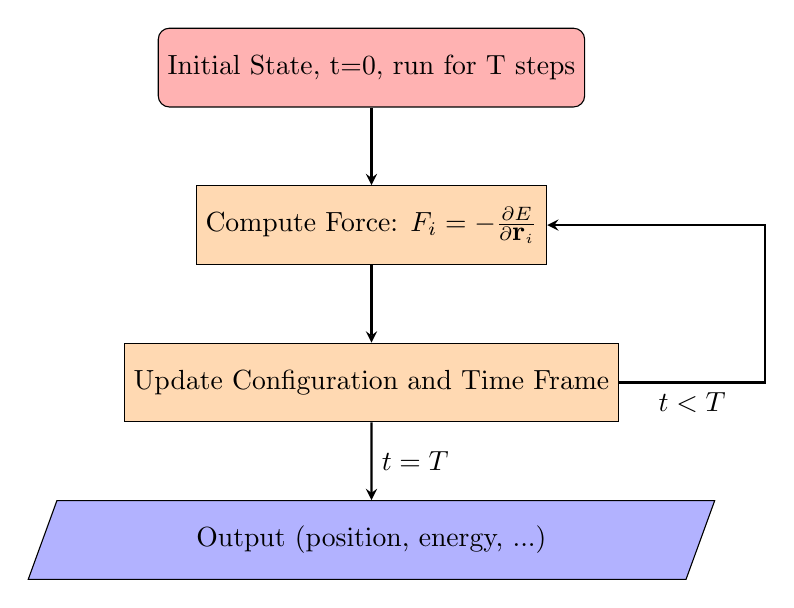
\begin{tikzpicture}[node distance=2cm]
\node (start) [startstop] {Initial State, t=0, run for T steps}; 
\node (pro1) [process, below of=start] {Compute Force: $F_{i}=-\frac{\partial E}{\partial \textbf{r}_i}$}; 
\node (pro2) [process, below of=pro1] {Update Configuration and Time Frame}; 
%\node (dec1) [decision, below of=pro2, yshift=-0.5cm] {Decision 1}; 
\node (out1) [io, below of=pro2] {Output (position, energy, ...)};	
\draw [arrow] (start) -- (pro1);
\draw [arrow] (pro1) -- (pro2);
\draw [arrow] (pro2) -- node[anchor=north]{$t<T$} ++(5,0) |- (pro1);
\draw [arrow] (pro2) -- node[anchor=west]{$t=T$} (out1);
\end{tikzpicture}
\end{frame}

\begin{frame}{Calculating molecular interactions $E$}
Total energy can be calculated as
\begin{equation}
E_{total} = E_{bonded} + E_{nonbonded}, 
\end{equation}
\ which consists of bonded interactions, 
\begin{equation} 
E_{bonded} = E_{bonds} + E_{angles} + E_{dihedrals}, 
\end{equation}
\ and nonbonded interactions, 
\begin{equation}
E_{nonbonded} = E_{electrostatic} + E_{vdW}. 
\end{equation}
Update frame as 
\begin{equation}
r(t+1) = r(t) + v(t) dt + \frac{1}{2} a(t) dt^2
\end{equation}
\end{frame}

%\begin{frame}{An Example}
%\begin{figure}
%	\includegraphics[width=\linewidth]{Pics/LYS.png}
%	\caption{Single molecular activity of lysozymn adsorption on graphene surface in atomstic resolution.   }
%\end{figure}
%\hfill {\tiny C.M. Nakano, H. Ma et al. \emph{Comp. Phys. Comm.} \textbf{2015}, 193, 1. }
%\end{frame}


\begin{frame}{Applications} 
\begin{quote}
	Everything that living things do can be reduced to wiggling and jiggling of atoms. 
	\\ \hfill --Richard Feynman (1963)
\end{quote}
\vspace{-.5cm}
\begin{figure}
	\includegraphics[width=.9\linewidth]{Pics/scale_comm.jpg}
%	\caption{MD scale}
\end{figure}
\end{frame}
% Need to cover simulation scale and application on physiological (learning from the nature) 
%, bioenergy, biomedical, and biosensing. 
	
\subsection{Free Energy Computation}
\begin{frame}{Free Energy}
To identify the thermodynamic favorability and spontaneousness of a given physical process, 
\vspace{1cm}
\begin{itemize}
	\item 
	Free Energy, 
	\begin{equation}
	G = H - TS. 
	\end{equation}

	\item Statistical Mechanics, 
	\begin{equation}
	G = - k_B T ln Q
	\end{equation}
\end{itemize}	

\end{frame}





%\section{Research Projects}
\subsection{Study of Protein Conduit on Electrode Surface}
\begin{frame}{Decaheme Cytochrome MtrF protein } 
	Originally from metal-reducing bacteria, \emph{Shewanella Oneidensis}. 
	\begin{figure}
		\includegraphics[width=\linewidth]{Pics/MtrF.png}
		\caption{SEM image of \emph{Shewanella Oneidensis} and its extracellular nanowires (a) and the hypothetic model of the protein conduit structure (b,c). }
	\end{figure} 
	\hfill {\tiny C.M. Nakano, H. Ma et al. \emph{Comp. Phys. Comm.} \textbf{2015}, 193, 1.
	}
\end{frame}

\begin{frame}{Simulation system}
	\begin{columns}
		\column{.6\linewidth}
		\begin{figure}
			\includegraphics[width=\columnwidth]{Pics/MtrF_path.png}
			\caption{Au(111) surface and MtrF protein with ET pathway}
		\end{figure}
		\column{.5\linewidth} 		
			MtrF protein (3pmq) 
				\begin{enumerate}
					\item Four distinct domains
					\item ET network formed by heme groups
				\end{enumerate}   
			Gold (111) surface 
			\begin{enumerate}
				\item Popular electrode material
				\item Strong interaction with protein
				\item Unique Au-S bond
			\end{enumerate}
		\vspace{2cm}
		{\tiny T. Wei, H. Ma et al. \emph{J. Phys. Chem. Lett.} \textbf{2016}, 7, 929.}
	\end{columns}
\end{frame}

\begin{frame}{Motivations \& Challenges}
	Motivations: 
	\begin{enumerate}
		\item Understand the unique mechanism of electron transfer (ET) through MtrF
		\item Explore and facilitate application of MtrF coated electrodes
	\end{enumerate}
	\begin{columns}
		\column{.5\linewidth}
		\begin{figure}
			\includegraphics[width=\columnwidth]{Pics/MtrF_path.png}
			\caption{Au(111) surface and MtrF protein with ET pathway}
		\end{figure}
		\column{.6\linewidth} 
		Challenges:
		\begin{enumerate}
			\item ET is highly depending on the orientation and structural stability of the MtrF protein. 
			\item The protein is large. 
			\item Slow rotation in classic atomistic MD simulation
			\item Possibly large attraction between protein and Au(111) surface 
		\end{enumerate} 
	\end{columns}
\end{frame}

\begin{frame}
\frametitle{Scheme}
\begin{columns}
\column{.6\linewidth}
\begin{figure}
	\includegraphics[width=\columnwidth]{Pics/MtrF_path.png}
	\caption{Au(111) surface and MtrF protein with ET pathway}
\end{figure}
\column{.5\linewidth}
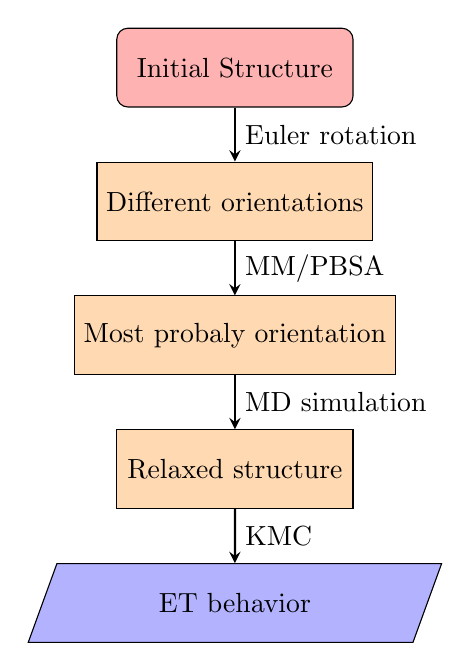
\begin{tikzpicture}[node distance=1.7cm]
\node (start) [startstop] {Initial Structure}; 
\node (pro1) [process, below of=start] {Different orientations};
\node (pro2) [process, below of=pro1] {Most probaly orientation}; 
\node (pro3) [process, below of=pro2] {Relaxed structure}; 
%\node (dec1) [decision, below of=pro2, yshift=-0.5cm] {Decision 1}; 
\node (out1) [io, below of=pro3] {ET behavior};	
\draw [arrow] (start) -- node[anchor=west]{Euler rotation} (pro1);
\draw [arrow] (pro1) -- node[anchor=west]{MM/PBSA} (pro2);
\draw [arrow] (pro2) -- node[anchor=west]{MD simulation} (pro3);
\draw [arrow] (pro3) -- node[anchor=west]{KMC} (out1);
\end{tikzpicture}
\end{columns}
\end{frame}

%\subsubsection{MM/PBSA}
\begin{frame}{MM/PBSA}
Molecular Mechanics/Poisson Boltzmann Surface Area 
\vspace{-.5cm}
\begin{figure}
	\centering
	\includegraphics[width=.5\textwidth]{Pics/MMPBSA.png}
\end{figure}
\vspace{-.7cm}
\centering
\begin{eqnarray}
	\Delta G_{binding} &=& G_{aqu}^{AB}- G_{aqu}^{A} - G_{aqu}^{B} \\
	G_{aqu}^{i} &=& G_{gas}^i + \Delta G_{sol}^i, i=A,B\ and\ AB \\
	G_{gas}^{i} &=& E_{bonded}^{i} + E_{LJ}^{i} +E_{coul}^i - T \cdot S^i\\
	\Delta G_{sol}^i &=& \Delta G_{polar}^i + \Delta G_{nonpolar}^i\\
	\Delta G_{polar}^i &=& G_{polar, \varepsilon = 80}^i - G_{polar, \varepsilon=1}^i\\
	\Delta G_{nonpolar}^i &=& \gamma _i \langle SASA_i \rangle
\end{eqnarray} 
Solvation energy consists of both long-range electrostatic and short-range surface tension contributions.
\end{frame}

\begin{frame}
\frametitle{MM/PBSA result}
\vspace{-.7cm}
\begin{figure}
	\includegraphics[width=.9\linewidth]{Pics/MtrF_MMPBSA.png} 
	\caption{Free energy profile (left) of MtrF on Au(111) surface according to 2nd and 3rd Euler angle with marked most probable configurations (right).}
\end{figure}
\begin{itemize}
	\item Four selected configurations are obtained according to binding energy. 
	\item Configuration (1) with heme 5 on the surface is picked for further MD simulation. 
\end{itemize}

\end{frame}

\begin{frame}
\frametitle{MD simulation result} 
MD simulation was run for 200 ns ($200 \times 10^6$ time steps). 
\begin{figure}
	\includegraphics[width=\linewidth]{Pics/MtrF_MD.png}
	\caption{Initial (left) and relaxed structure (right) of MtrF on Au(111) surface.}
\end{figure}
\begin{itemize}
	\item Heme network is preserved through MD relaxation. 
	\item Domain III is adsorbed unto the surface. 
	\item Au-S interaction restrains the protein lateral diffusion. 
\end{itemize}
\end{frame}

%\subsection{Kinetic Monte Carlo (KMC) simulation}
\begin{frame}{Kinetic Monte Carlo (KMC) simulation}
Define Monte Carlo moves of electron transfer in MtrF protein
\begin{figure}
	\centering
	\includegraphics[width=\textwidth]{Pics/KMC_move.png}
\end{figure}
\end{frame}

\begin{frame}{Kinetic Monte Carlo (KMC) simulation}
At each step, 
\begin{enumerate}
\item Sum up all M possible events according to the electron network redox condition
\begin{equation}
	k_{total} = \sum_{l=1}^{M} k_l
\end{equation}
\item Select specified event $l^*$ by random operation, 
\begin{equation}
	\sum_{l=1}^{l^* -1} k_l < \xi_1 k_{total} < \sum_{l=1}^{l^*} k_l,\ (0<\xi_1<1)
\end{equation}
\item Apply time increment, $\tau = - ln(\xi_2)k_{total}^{-1}$
\end{enumerate}
%The neighbor hoping rate was calculated by 
%\begin{equation}
%k_{ij} = \frac{2 \pi}{h} \langle|H_{ij}|^2\rangle \frac{1}{\sqrt{4 \pi \lambda k_B T}} exp\left( -\frac{(\Delta G_{ij} + \lambda)^2}{4 \lambda k_B T} \right)
%\end{equation}
\end{frame}

\begin{frame}
\frametitle{KMC result}
%Anode gold surface (Electron transfers from heme 5 to 10, i.e. surface to solution). 
\begin{figure}
	\includegraphics[width=\linewidth]{Pics/MtrF_KMC.png} 
	\caption{Phase diagrams of time-averaged electron occupation density (a,c) and flow rate (b,d) as function of incoming ($\alpha$) and outgoing ($\beta$) rate.}
\end{figure}
%\begin{itemize}
%	\item Three distinct regions: Low-density (LD), High-density (HD) and Maximum current (MC). 
%\end{itemize}
\end{frame}

\begin{frame}
\frametitle{Conclusions}
\begin{itemize}
	\item MD simulation were applied to obtain the steady state of biophysical system. 
	\item Various methods of free energy calculation were adopted to understand certain biophysical processes.  
	\item Structural stability and acyl hydrophobicity affects the water passive permeation through the bilayer membrane of Lipid A and its analogue.  
	\item Adosption of MtrF protein on Au(111) surface is highly influenced by strong surface tension. 
	\item MtrF protein has different electron resistances under current flowing in reverse direction. 
\end{itemize}
\end{frame}

%\subsection{DNA SAM Surface Morphology Study for Cancer Diagnosis}
%\begin{frame}{DNA SAM surface for cancer diagnosis}
%
%{\bf Experimental Design}
%\begin{figure}
%	\centering
%	\includegraphics[width=\linewidth]{Pics/dna_sam.png}
%	\caption{DNA SAM surface morphology (left) and workflow scheme (right) for evaporating droplet array and probe-target hybridization. }
%\end{figure}
%\vspace{-.5cm}
%	\hfill {\tiny Q. Wen, I. Lian et al. \emph{. Ann. Biomed. Eng.} \textbf{2014}, 42.9, 1932.}
%\end{frame}
%
%\begin{frame}{MD simulation system}
%MD simulation was set up on $\alpha$-cristobalite (101) surface in dimension of 13.68$\times$ 12.94 nm$^2$. 
%
%\begin{columns}
%\column[]{.4\linewidth}
%\begin{figure}
%	\includegraphics[width=\columnwidth]{Pics/DS11.png}
%\end{figure}
%\column[]{.85\linewidth}
%\begin{itemize} 
%%	\item Surface probe grafting density
%%	\begin{tabular}{c | c | c}
%%		\hline
%%		Number of probes & $\rho_{grafting}$ (/cm$^2$) & Label \\
%%		\hline
%%		1 & $0.565 \times 10^{12}$ & DS1  \\
%%		\hline
%%		4 & $2.26 \times 10^{12}$ & DS4 \\
%%		\hline
%%		9 & $5.08 \times 10^{12}$ & DS9 \\
%%		\hline
%%	\end{tabular}	
%	\item Probe hybridization state \\
%		Influence of double-strand helical structure
%	\item Cation concentration and type \\
%	\begin{tabular}{c|c|c|c|c}
%		\hline
%		Cation type & \multicolumn{4}{|c}{Concentration (mol/L)} \\
%		\hline
%		$Na^+$ & Counterion & 0.15 & 0.6 & 1.0 \\
%		\hline
%		$Mg^{2+}$ & & 0.15 & & 1.0 \\
%		\hline
%	\end{tabular}
%%	\item Sample concentration and purity
%\end{itemize}
%\end{columns}
%\end{frame}
%
%%\begin{frame}{Grafting density and hybridization state}
%%	\begin{figure}
%%		\centering
%%		\includegraphics[width=\linewidth]{Pics/dna_gd.png}
%%		\caption{Z-axis density profile of DNA SAM surface under various grafting densities and hybridization states}
%%	\end{figure}
%%\end{frame}
%
%\begin{frame}{Radial distribution of $Na^+$ around ssDNA and dsDNA}
%\begin{columns}
%	\column[]{.45\linewidth}
%	\begin{figure}
%		\includegraphics[width=\columnwidth]{Pics/dna_gd_rdf.png}
%		\caption{\scriptsize Proximal radial concentration of $Na^+$ in 0.15 M NaCl solution. }
%	\end{figure}
%
%	\column[]{.6\linewidth}
%	\begin{figure}
%		\includegraphics[width=\columnwidth]{Pics/dna_na.png}
%		\caption{\scriptsize Two types of $Na^+$ cations associating with DNA. }
%	\end{figure}
%	\begin{itemize}
%		\item High cation concentration around the ssDNA. 
%		\item $Na^+$ cations preferably associate directly with ssDNA, and through water shell with dsDNA. 
%	\end{itemize}
%\end{columns}
%\end{frame}
%
%\begin{frame}{Ion concentration influences}
%\begin{figure}
%	\includegraphics[width=.85\linewidth]{Pics/dna_ion.png}
%	\caption{$H=5.52 \times exp(-C/0.13) + 4.67$}
%\end{figure}
%\vspace{-.5cm}
%{\footnotesize where H is the height of DNA layer and C is concentration of NaCl.} 
%\end{frame}
%
%\begin{frame}{$Na^+$ condensation equilibrium}
%To quantify the amount of DNA charge neutralized by solution ions, an equilibrium is purposed as 
%\begin{equation}
%Na^+_{bulk} + Na_m DNA^{-(n-m)} \Longleftrightarrow Na_{m+1} DNA^{-(n-m-1)}
%\end{equation}
%Percentage of neutralized DNA charge base on Manning's Counterion Condensation theory: 
%\begin{equation}
%n_{ex} = \frac{\sum_{r=0}^{r<0.9nm} [N_{Na^+}(r) - N_{Cl^-}(r)]}{Q_{DNA}}
%\end{equation}
%The result was \\
%\vspace{.1cm}
%\begin{tabular}{c|c|c|c|c}
%	$C_{NaCl}$ (mol/L) &  Counterion & 0.15 & 0.6 & 1.0\\
%	\hline
%	$n_{ex}$ & 71.5\% & 85.1\% & 93.7\% & 98.7\% \\
%\end{tabular}
%\end{frame}
%
%\begin{frame}{$Mg^{2+}$ v.s. $Na^+$}
%\begin{figure}
%	\includegraphics[width=\linewidth]{Pics/dna_mg.png}
%	\caption{Different from $Na^+$, $Mg^{2+}$ cations associate with DNA through hydration water clusters. }
%\end{figure}
%\end{frame}
%
%
%\begin{frame}{Conclusions}
%\begin{itemize}
%	\item DNA SAM surface with higher packing density exhibits less meltdown of nucleic chains. 
%	\item ssDNA melts down into a mushroom-like coil and dsDNA maintains a rod-like helical structure. 
%	\item Cations in the solution can neutralize the negative charge from DNA and induce further meltdown. 
%	\item Cations associated with DNA through two main ways: direct contact and water mediated association. 
%\end{itemize}
%\end{frame}

\section{Machine Learning Piloting Simulations} 
\subsection{Applications}
\begin{frame}{Machine Learning and Artificial Intelligence}
{Development and Applications} 
{\centering From Bombe to Alpha Go and far beyond \par } 
\begin{figure}
	\includegraphics[width=.8\linewidth]{Figures/Figure_AI.png} 
%	\includegraphics[width=.3\linewidth]{./Pics/Nature-Go-game-cover.jpg} \\
%	\includegraphics[width=\linewidth]{Pics/machine-learning.png}

\end{figure}
\end{frame}


\begin{frame}{Machine Learning}
\begin{figure}
		\includegraphics[width=.9\linewidth]{Pics/machine-learning.png}
\end{figure}
\end{frame} 

\subsection{Convolutional Variational Autoencoder}
\begin{frame}{Convolutional Variational Autoencoder (CVAE)}
\begin{figure}
	\includegraphics[width=\linewidth]{Pics/CVAE.png} 
%	\caption{Convolutional variational autoencoder architecture}
\end{figure} 
\vfill 
\hfill {\tiny D. Bhowmik, et al. BMC Bioinformatics, 2018, 19 (Suppl 18) :484}
\end{frame}

\subsection{CVAE-piloting MD simulations}
\begin{frame}{CVAE-piloting MD simulations }
\begin{figure}
	\includegraphics[width=\linewidth]{Pics/MicroScope_Workflow_Diagram.pdf} 
	%	\caption{Convolutional variational autoencoder architecture}
\end{figure}
\end{frame}


\begin{frame}
\frametitle{Setup for Workflow} 
\begin{itemize}
	\item \textbf{MD simulation}: OpenMM   \\
%	\hspace{3cm}	\includegraphics[width=1cm]{Pics/OpenMM.png} 
	\item \textbf{Machine Learning}: Keras/Tensorflow \\
%		\hspace{3.25cm}	\includegraphics[width=1cm]{Pics/Keras_logo.jpg}  
%		\includegraphics[width=1cm]{Pics/TF_logo.png}
	\item \textbf{Scheduler}: Celery, Radical.entk
	\item \textbf{Hardware}: GPU platforms \\ 
	\vspace{.3cm}
	Tested on dgx2 from CADES-ornl. \\
	\begin{itemize}
		\item 16 $\times$ Nvidia Tesla V100-SXM3-32GB 
		\item 21-AA fs-peptide 
		\item 28 MD simulation runs
	\end{itemize}
\end{itemize}
\end{frame} 

\begin{frame}
\frametitle{Running the workflow} 
\href{./Figures/CVAE_MD.html}{Let's see the code. } 
%\href{file://./Figures/CVAE_MD.html}{Let's see the code. }
\end{frame} 


\begin{frame}{MD simulation results} 
\begin{figure}
	\includegraphics[width=\textwidth]{Figures/RMSD_MD.png} 
	\caption{RMSD profile of 28 MD simulations managed by CVAE} 
\end{figure} 
\end{frame} 

\begin{frame}
\frametitle{Latent space view}  
\href{./Figures/CVAE_3d_plot.html}{3D latent dimension CVAE results }
\begin{itemize}
	\item 
	\href{./Figures/cm_predict.html}{Every 10 frames} 
	\item 
	\href{./Figures/cm_predict_first_100k.html}{First 100,000 conformers}
	\item 
	\href{./Figures/cm_predict_last_100k.html}{Last 100,000 conformers}
	\item 
	\href{./Figures/cm_predict_outliers.html}{Outliers} 
\end{itemize}

\end{frame}


\begin{frame}{Conformational analysis} 
\href{./Figures/cm_predict.html}{3D latent space} 
\begin{figure}
	\includegraphics[width=\linewidth]{Figures/Gephi_save_2k_crop.png} 
	%	\caption{Convolutional variational autoencoder architecture}
\end{figure}
\end{frame}
%\section{Future Plans}
%\begin{frame}{What is next?}
%\centering
%I propose to consider the question, `Can machines think?'
%	\begin{figure}
%		\includegraphics[width=.5\linewidth]{Pics/aturing.jpg}
%		\caption{Alan Turing}
%	\end{figure}
%Can machine do all these things above? 
%\end{frame}
%
%\begin{frame}{Computational drug discovery workflow}
%\begin{columns}
%	\column[]{.3\linewidth}
%	\begin{tikzpicture}[node distance=2cm]
%	\node (start) [startstop] {Source}; 
%	\node (pro1) [process, below of=start] {Candidates \emph{in silico}}; 
%	\node (pro2) [process, below of=pro1] {Screening }; 
%	%\node (dec1) [decision, below of=pro2, yshift=-0.5cm] {Decision 1}; 
%	\node (out1) [startstop, below of=pro2] {Candidates \emph{in vitro}};	
%	\draw [arrow] (start) -- (pro1);
%	\draw [arrow] (pro1) -- (pro2);
%	\draw [arrow] (pro2) -- ++(2,0) |-(pro1);
%	%\draw [arrow] (pro2) -- node[anchor=north]{$t<T$} ++(5,0) |- (pro1);
%	%\draw [arrow] (pro2) -- node[anchor=west]{$t=T$} (out1);
%	\draw [arrow] (pro2) -- (out1);
%	\end{tikzpicture}
%	
%	\column[]{.7\linewidth}
%	\begin{enumerate}
%		\item Source \\
%		Natural source, small molecule library,``me too" drugs,...
%		\vspace{.4cm} 
%		\item Designing candidates base on Structure-Activity Relation (SAR) 
%		\vspace{.4cm}
%		\item Screening \\
%		\begin{itemize}
%			\item MD simulation and free energy assessment (force field parameters)
%			\item High Throughput Screening (HTS) base on physico-chemical properties
%		\end{itemize}
%		\vspace{.4cm}
%		\item Lead and backup compounds for \emph{in vitro} testing
%	\end{enumerate}
%\end{columns}
%\end{frame}
%
%\begin{frame}{MD simulation in screening process} 
%Processes and challenges to build the workflow: 
%\begin{enumerate}
%	\item Obtain the compound configuration from docking models\\
%	Selecting the ideal candidate from docking result
%	\item Choose a force field \\
%	Assigning the parameters for the small molecules 
%	\item MD simulation in solvent environment \\
%	Automatic system setup and simulation monitoring
%	\item Calculate binding free energy\\
%	$\Delta G_{binding} = \Delta G_{configuration} + \Delta G_{desolvation} + \Delta G_{interaction}$ \\
%	Taking MD results into free energy algorithm
%	\item Select the lead compound 
%	\item Fault recovery	
%\end{enumerate}
%%force field -> MD simulation -> Binding free energy
%\end{frame}
%
%\begin{frame}{Computer-aided High-Throughput Screening}
%What if we have more candidates? Amount like 10000?
%\begin{figure}
%	\includegraphics[width=\linewidth]{Pics/DrugDis.jpg}
%\end{figure}
%\vspace{-.3cm}
%Structure-Activity Relation based Machine Learning
%\begin{figure}
%	\includegraphics[width=.6\linewidth]{Pics/DecisionTree.jpg}
%\end{figure}
%%SAR that assess candidate characteristics can be derived from sufficient MD simulation cases (both literature and local)
%\end{frame}
%
%\begin{frame}
%Molecular properties \hfill ADMET properties
%\begin{figure}
%	\includegraphics[width=.9\linewidth]{Pics/MLDD.jpg}
%\end{figure}
%\end{frame}
%
%\begin{frame}{Computational proteome study}
%Proteome is an entire set of proteins expressed by a genome in certain time. \\
%\vspace{1cm}
%Motivation: 
%\begin{itemize}
%	\item Interaction network
%	\item Biomarker for diagnostics
%	\item Proteogenomics
%	\item Structural proteomics
%\end{itemize}
%
%%System biology
%%Protein identification
%%SAR study
%\end{frame}
%

%
%%\begin{frame}{Challenges}
%%Biological complexity: 
%%\begin{itemize}
%%	\item Alternative splicing \\
%%	More than one protein risen from a single transcript
%%	\item Post-translational modifications \\
%%	Phosphorylation, Ubiquitination, methylation, acetylation, oxidation, ...
%%	\item Genetic information from RNA
%%	\item DNA/RNA aptamer
%%	\item Solvent effects
%%	\item Dynamical system
%%\end{itemize}
%%Computational challenge: 
%%\begin{itemize}
%%	\item Size of proteome encoded in genome \\
%%	136,594 protein structures in Protein Data Bank (rcsb.org)
%%\end{itemize}
%%\end{frame}
%
%\begin{frame}{Long-term plan}
%\begin{columns}
%	\column[]{.3\linewidth}
%	\begin{tikzpicture}[node distance=2cm]
%	\node (start) [process] {Genome}; 
%	\node (pro1) [process, below of=start] {Transcriptome}; 
%	\node (pro2) [process, below of=pro1] {Proteome}; 
%	%\node (dec1) [decision, below of=pro2, yshift=-0.5cm] {Decision 1}; 
%	\node (out1) [process, below of=pro2] {Protein };	
%	\draw [arrow] (start) -- (pro1);
%	\draw [arrow] (pro1) -- (pro2);
%	%\draw [arrow] (pro2) -- ++(2,0) |-(pro1);
%	%\draw [arrow] (pro2) -- node[anchor=north]{$t<T$} ++(5,0) |- (pro1);
%	%\draw [arrow] (pro2) -- node[anchor=west]{$t=T$} (out1);
%	\draw [arrow] (pro2) -- (out1);
%	\end{tikzpicture}
%	\column[]{.7\linewidth}
%	To identify the hidden algorithm via machine learning, it requires
%	\begin{itemize}
%		\item Variables to capture the hidden algorithm\\
%		Knowledge about the proteomics
%		\item Training data\\
%		Literature, database, ...
%		\item High performance computing
%		\item Verification 
%	\end{itemize}
%\end{columns}
%%\begin{figure}
%%	\includegraphics[width=\linewidth]{Pics/grp.png}
%%\end{figure}
%\end{frame}

\section{Proteome-scale Structure Prediction Workflow}   
\begin{frame}{High Throughput Proteome-Scale Structure Prediction}
\vspace{-.5cm}
\begin{figure}
	\includegraphics[width=\linewidth]{Pics/proteome}
\end{figure}
Average size of proteomes according to Proteome-\emph{pI} database
\begin{tabular}{c|c|c|c|c}
	\hline
	Species & Virus & Archaea & Bacteria & Eukaryotes \\
	\hline
	Proteome Size & 42 & 2,358 & 3,200 & 15,145 \\
	\hline
\end{tabular}

\vspace{.5cm}
\hfill {\tiny Lukasz P. Kozlowski, \emph{Nucleic Acids Res} \textbf{2017}, 45, D1112.}
\end{frame}

\begin{frame}{Workflow Overview}
\begin{enumerate}
	\item Initialize project 
	\item Gather target sequences from Uniprot or user input 
	\item Query homologous templates using hhblits 
	\item (Optional) Loopmodel to complete missing loops in template structure
	\item Homology modeling using RosettaCM protocol 
	\item MD simulations for structural refinement 
	\item Final structure for longer production MD simulations
\end{enumerate}
\end{frame}

\begin{frame}[fragile]
\begin{minted}[fontsize=\footnotesize]{python}
import hh_rose

hh_rose.build_env.Proj_Init()

query_string = 'PK3CA_HUMAN'
hh_rose.GatherTargetsFromUniprot(query_string)
# hh_rose.WriteTargetFromSequence('example', 'AAAAAAAAAA')

uniprot_dbs = '../../dbs/uniclust30_2018_08/uniclust30_2018_08'
pdb_dbs = '../../dbs/pdb70/pdb70'
hh_rose.gather_templates_from_sequence(
	uniprot_dbs=uniprot_dbs, pdb_dbs=pdb_dbs, n_cpus=24)

hh_rose.modeling.template_loopmodels(number_of_models=24, mpi_size=24)

hh_rose.modeling.build_models(number_of_models=1000, mpi_size=24, 
	number_of_selected=2, random_seed=12345678)

hh_rose.refinement.refine_implicit_md(gpupn=2)
hh_rose.refinement.refine_explicit_md(gpupn=2)

hh_rose.packaging.package_for_md()

\end{minted}
\end{frame}

\subsection{PK3CA\_HUMAN}
\begin{frame}{PK3CA\_HUMAN}
\begin{itemize}
	\item {
		Human kinase enzyme for phosphorylation
	}
	\item 
	Closely associated with diabetes, leukemia and various cancers
	\item 
	1068 Amino Acids 
	\item Encoded by gene \texttt{PIK3CA}
	\item 
	Uniprot mnemonic label: \texttt{PK3CA\_HUMAN}
	\item Uniprot accession number: \texttt{P42336}
\end{itemize}
\end{frame}

\begin{frame}{Templates and alignments}
The homologous template: \texttt{4JPS\_A}
\begin{itemize}
\item Sequence matching  
\begin{table}[!ht]
	\centering 
	%  		\caption{{\bf Summary of mismatch residues between PK3CA\_HUMAN and 4JPS\_A.}} 
	\begin{tabular}{c|cc}
		Residue Number & PK3CA\_HUMAN & 4JPS\_A \\ \hline 
		232 & MET & LYS \\ 
		233 & LEU & LYS \\ 
		1068 & ASN & - \\ 
	\end{tabular}
	\label{4jps_ali}
\end{table}
\item PDB from RCSB \\
Four missing loops: LYS228-VAL243, ALA314-SER323, TRP498-ARG524, and GLY864-GLN871 
\item Loopmodel 
\end{itemize}
\end{frame}

% You can reveal the parts of a slide one at a time
% with the \pause command:
\begin{frame}{Rosetta Comparative Modeling}  
1000 decoys are produced in this step. 
\begin{figure}
\includegraphics[width=\linewidth]{./Figures/fig2.jpg}
\end{figure} 
S\_0066 and S\_0873 are the top 2 models for further refinements. 
\end{frame}


\begin{frame}{MD refinements} 
Two steps: 
\begin{enumerate}
\item 10-ps Implicit MD simulation 
\item 1-ns Explicit MD simulation 
\end{enumerate} 

\begin{columns}
\begin{column}{0.6\textwidth} 
\begin{itemize} 
\item
Solvation: \\ \hspace{.1in}  Padding distance = 10 \AA. 
\begin{tabular}{c|cc} 
	\hline
	Systems & Edge Length & \# of H\textsubscript{2}O\\ \hline
	S\_0066 & 128.755 & 62139 \\
	S\_0873 & 136.887 & 76311 \\ \hline
\end{tabular} 
\item 
Relaxation (right): \\
The system is able to reach lower energy states. 
\end{itemize}
\end{column} 

\begin{column}{0.4\textwidth}  %%<--- here
\begin{figure}
\includegraphics[width=\linewidth]{./Figures/Energy.jpg}
\end{figure}
\end{column} 
\end{columns}
\end{frame}

\begin{frame}{Performance}
\begin{figure}
\includegraphics[width=\linewidth]{./Figures/Result_run_time.png} 
\caption{The run time of stages in the workflow, 3.4 core hours per decoy. }
\end{figure}

\end{frame}

\subsection{HIV-1MB proteome} 

\begin{frame}{HIV-1MB Proteome and templates}
\begin{table}[!ht] 
	\centering 
	%		\caption{{\bf Summary of HIV-1MB proteome target sequences and homologous templates. } } 
	\begin{tabular}{ccl}
		Protein & Length & Templates\\ \hline 
		REV\_HV1H2 & 116 & 5DHX\_C (1-65) \\
		POL\_HV1H2 & 1435 & 1ED1\_A (1-132), 5UP4\_A (133-353),  \\
		&& 1BAI\_A (496-586), 1MU2\_A (591-1142),  \\
		&& 3F9K\_U (1149-1351), 4FW1\_B (1201-1416) \\
		TAT\_HV1H2 & 86 & 3MI9\_C (1-86) \\
		VIF\_HV1H2 & 192 & 4N9F\_b (1-176) \\
		VPU\_HV1H2 & 81 & 2JPX\_A (1-36), 2N29\_A (28-81)\\
		VPR\_HV1H2 & 96 & 1M8L\_A (1-96)\\
		GAG\_HV1H2 & 500 & 1ED1\_A (1-132), 2C55\_A(449-500), \\
		&& 3GV2\_F (133-366), 5UP4\_H (133-353)\\ 
		&& {\color{red} 5KP9\_B (429-500)}\\
		ENV\_HV1H2 & 856 & 4JZZ\_A(20-492), 6B0N\_G(32-664)\\
		&&{\color{red} 6DCQ\_D(514-856)}\\
		NEF\_HV1H2 & 206 & 3TB8\_A (1-206)\\
	\end{tabular}  
	\label{HIV-prot}  
\end{table}
\end{frame}


\section{Future Plan}
\begin{frame}{Future Plan}
Application of AI/ML methods in 
\begin{itemize}
	\item Protein-protein interaction network 
	\item Small molecule network for drug design \& discovery 
\end{itemize}
\end{frame}

\begin{frame}{Protein-protein interaction network} 
%Challenges: 
%\begin{itemize}
%	\item 
%\end{itemize}
\begin{figure}
	\includegraphics[width=\linewidth]{Pics/PPI_network.jpg} 
	\caption{Predicted protein interaction network of fission yeast. }
\end{figure}
\vfill \hfill {\tiny V. Pancaldi, G3: GENES, GENOMES, GENETICS, 2012, 2 (4) 453-467}
\end{frame}

\begin{frame}{AI/ML interfacing} 
Transfer knowledge-based experimental design to data-based
\begin{figure}
	\includegraphics[width=.7\linewidth]{Pics/Exp_AI.png}
\end{figure} 
\begin{itemize}
	\item The experiments provides validation and training input 
	\item The AI/ML models design experiments   
\end{itemize} 
\end{frame}


\begin{frame}{Summary}
\begin{itemize}
	\item Previous study of MD simulation and free energy calculation was carried out to understand biophysical process. 
	\item Machine Learning models interfaces with MD simulations runs to probe rare conformations/events. 
	\item Protein structure prediction workflow is designed for proteome scale study.  
	\item AI/ML frameworks are proposed to exploit complex experimental result for adaptive experiment design. 
\end{itemize}
\end{frame}

\begin{frame}{Acknowledgment}
\vspace{-.5cm}
\begin{columns}
	\column{.6\linewidth} 
	Adviser: \\ 
	\hspace{.5 cm} Dr. Arvind Ramanathan \\
	\hspace{.5 cm} Dr. Jeremy Smith \\
	\hspace{.5 cm} Dr. Tao Wei (Howard U.)\\ 
	Collaborators: \\ 
	\hspace{.5 cm} Dr. Debsindhu Bhowmik \\
	\hspace{.5 cm} Dr. Jerry Parks \\ 
	\hspace{.5 cm} Dr. Christopher Stanley \\
	\hspace{.5 cm} Dr. Aiichiro Nakano (USC)\\
	\hspace{.5 cm} Dr. Mohamed Y. El-Naggar (USC)\\
	
	\column[]{.4\linewidth}
	\begin{figure} 
		\includegraphics[width=.8\columnwidth]{Pics/ORNL.png} \\ 
		\includegraphics[width=.8\columnwidth]{Pics/cmb_logo.png} \\
		\includegraphics[width=.5\columnwidth]{Pics/LU.jpg} \\
		\includegraphics[width=.8\columnwidth]{Pics/TACC.png} \\
		\includegraphics[width=.8\columnwidth]{Pics/XSEDE.png}
		
	\end{figure}
	
\end{columns}

\end{frame}

\begin{frame}
 \centering 
 {\Large Thank you}
\end{frame}
\end{document}
 

